% uncomment this to use pubform
%\documentstyle[psfig, amsmath]{pubform}

\documentclass{sig-alternate}
\usepackage{gregs-defs}

\begin{document}

% need this on cagfarm's besides cagfarm-01
%\advance\topmargin by 1in

\title{StreamIt: A Compiler for Streaming Applications\thanks{This document is MIT Laboratory for Computer Science Technical Memo LCS-TM-622, February, 2002.}}

% uncomment this to use pubform
%% \author{Bill Thies, Michal Karczmarek, Michael Gordon, David Maze, Jeremy Wong, \\ Henry Hoffmann, Matthew Brown, and Saman Amarasinghe \\
%% \parbox{6in}{\centering{Laboratory For Computer Science\\
%%     Massachusetts Institute of Technology\\
%%     Cambridge, MA  02139\\
%%     \tt{\{thies, karczma, mgordon, dmaze, jnwong, hank, morris, saman\}@lcs.mit.edu}}}}
%% \date{\today}

\numberofauthors{1}
\author{
\alignauthor \vspace{-18pt}
William Thies, 
Michal Karczmarek, 
Michael Gordon, 
David Maze, 
Jeremy Wong,
Henry Hoffmann, 
Matthew Brown, 
and Saman Amarasinghe\\
	\vspace{8pt}
	\{thies, karczma, mgordon, dmaze, jnwong, hank, morris, saman\}@lcs.mit.edu \\
	\vspace{8pt}
	Laboratory for Computer Science \\
	Massachusetts Institute of Technology \\
	Cambridge, MA  02139 \\
	\vspace{8pt}
        February 12, 2002}
	
%        \today

% for the arrow of a function def, etc.
\newcommand{\ma}[2]{max_{#1 \rightarrow #2}}
\newcommand{\sdep}[0]{\textsc{sdep}}
\newcommand{\loopdep}[0]{\textsc{loopdep}}
\newcommand{\mi}[2]{\sdep_{#2 \small{\rightarrow} #1}}
\newcommand{\floor}[2]{\left\lfloor\frac{#1}{#2}\right\rfloor}
\newcommand{\ceil}[2]{\left\lceil\frac{#1}{#2}\right\rceil}
\newcommand{\ra}[0]{\rightarrow}
\newcommand{\la}[0]{\lambda}

\def\fn#1{\mathop{\mbox{\it #1}}}
\def\fun#1#2{\ensuremath{\mathop{\mbox{\it #1}}(#2)}} % function call

\newtheorem{definition}{Definition}
\newtheorem{theorem}{Theorem}

\maketitle

\begin{abstract}
As DSP programming is becoming more complex, there is an increasing
need for high-level abstractions that can be efficiently compiled.
Toward this end, we present a set of aggressive optimizations that
target linear sections of a stream program.  Our input language is
StreamIt, which represents programs as a hierarchical graph of
autonomous filters.  A filter is linear if each of its outputs can be
represented as an affine combination of its inputs.  Linear filters
are common in DSP applications; examples include FIR filters,
expanders, compressors, FFTs and DCTs.

We present a linear extraction analysis that automatically detects
linear filters based on the C-like code in their {\tt work} function.
Once linear filters are identified, we show how neighboring nodes can
be collapsed into a single linear representation, thereby eliminating
many redundant computations.  Also, we describe a method for
automatically translating linear nodes into the frequency domain,
thereby yielding algorithmic savings for convolutional filters.

We have completed a fully-automatic implementation of the above
techniques as part of the StreamIt compiler, and we demonstrate
performance improvements that average 400\% over our benchmark
applications.




\end{abstract}

\section{Introduction}

Applications that are structured around some notion of a ``stream''
are becoming increasingly important and widespread.  There is evidence
that streaming media applications are already consuming most of the
cycles on consumer machines \cite{Rix98}, and their use is continuing
to grow.  In the embedded domain, applications for hand-held
computers, cell phones, and DSP's are centered around a stream of
voice or video data.  The stream abstraction is also fundamental to
high-performance applications such as intelligent software routers,
cell phone base stations, and HDTV editing consoles.

Despite the prevalence of these applications, there is surprisingly
little language and compiler support for practical, large-scale stream
programming.  Of course, the notion of a stream as a programming
abstraction has been around for decades \cite{SICP}, and a number of
special-purpose stream languages have been designed (see
\cite{survey97} for a review).  Many of these languages and
representations are elegant and theoretically sound, but they often
lack features and are too inflexible to support straightforward
development of modern stream applications, or their implementations
are too inefficient to use in practice.  Consequently, most
programmers turn to general-purpose languages such as C or C++ to
implement stream programs.

There are two reasons that general-purpose languages are inadequate for
stream programming.  Firstly, they are a mismatch for the application
domain.  That is, they do not provide a natural or intuitive
representation of streams, thereby having a negative effect on
readability, robustness, and programmer productivity.  Moreover, because
the widespread parallelism and regular communication patterns of data
streams are left implicit in general-purpose languages, compilers are
not stream-conscious and do not perform stream-specific optimizations.
As a result, performance-critical loops are often hand-coded in a
low-level assembly language and must be re-implemented for each target
architecture.  This practice is labor-intensive, error-prone, and very
costly.

Secondly, general-purpose languages are a mismatch for the emerging
class of grid-based architectures \cite{smartmemories,rawshort,trips} that
are especially well-suited for stream processing.  Perhaps the primary
appeal of C is that it provides a ``common machine language'' for
von-Neumann architectures.  That is, it abstracts away the
idiosyncratic differences between machines, but encapsulates their
common properties: a single program counter, arithmetic operations,
and a monolithic memory.  However, for grid-based architectures, the
von-Neumann model no longer holds, as there are multiple instruction
streams and distributed memory banks.  Thus, C no longer serves as a
common machine language--in fact, it provides the wrong abstraction
for the underlying hardware, and architecture-specific directives are
often needed to obtain reasonable performance.  Again, this greatly
complicates the job of the programmer and hampers portability.

StreamIt is a language and compiler specifically designed for modern
stream programming.  The StreamIt language has two goals: first, to
provide high-level stream abstractions that improve programmer
productivity and program robustness within the streaming domain, and
second, to serve as a common machine language for grid-based
processors.  At the same time, the StreamIt compiler aims to perform
stream-specific optimizations to achieve the performance of an expert
programmer.

This paper motivates, describes, and justifies the high-level language
features of StreamIt, version 1.0.  The major limitation of StreamIt
1.0 is that all flow rates in the streams must be static; applications
such as compression that have dynamically varying flow rates will be
the subject of future work.  A large set of applications can be
implemented with static rates, and while dynamic rates will require a
different runtime model, it will still be essential to fully analyse
and optimize static sub-sections in order to obtain high performance.

The paper is organized as follows. In Section {\ref{sec:domain}}, we
characterize the domain of streaming programs that motivates the
design of StreamIt, and in Section~\ref{sec:overview} we describe the
language features in detail.  We present an in-depth example of a
software radio in Section~\ref{sec:example}, preliminary results in
Section~\ref{sec:results}, related work in Section~\ref{sec:related},
and conclusions in Section~\ref{sec:conc}.


\section{StreamIt}
\label{sec:streamit}

StreamIt  is   an  architecture independent language that is
designed for  stream programming. In StreamIt, programs are
represented as graphs where  nodes represent  computation and edges
represent FIFO-ordered communication of data over tapes.

\paragraph*{Hierarchical Streams}
In  StreamIt, the  basic programmable  unit (i.e., an actor) is a {\it
filter}.   Each filter contains  a work  function that executes
atomically,  popping (i.e., reading)  a fixed number  of items  from
the  filter's input  tape and pushing (i.e., writing) a fixed number
of items to the filter's output tape.  A filter  may also {\tt peek} at
a given index  on its input tape without  consuming  the  item;  this
makes  it  simple  to  represent computation over a
sliding window.   The {\tt push}, {\tt pop}, and {\tt peek} rates are
declared as part  of  the work  function,  thereby enabling  the
compiler    to construct a static schedule of filter executions. The
following is an example implementation of a Finite Impulse
Response (FIR)  filter: 

\begin{scriptsize}
% {\small
\begin{verbatim}
float->float filter FIR (int N, float[] weights) 
{
  work push 1 pop 1 peek N {
    float sum = 0;
    for (int i = 0; i < N; i++) {
      sum += peek(i) * weights[i];
    }
    pop();
    push(sum);
  }
}
\end{verbatim}
% }
\end{scriptsize}

The work function is invoked (fired) whenever there is sufficient data
on the input tape. For the FIR example above, the filter requires at least
\texttt{N} elements before it can execute. The value of \texttt{N} is
known at compile time when the filter is composed to form a stream
graph. A filter is akin to a class in object oriented programming
with the work function serving as the main method. The parameters
to a filter (e.g., \texttt{N} and \texttt{weights}) are equivalent to
parameters passed to a class constructor. 

\begin{figure}[t]
\begin{center}
%\vspace{-24pt}
% \framebox{
 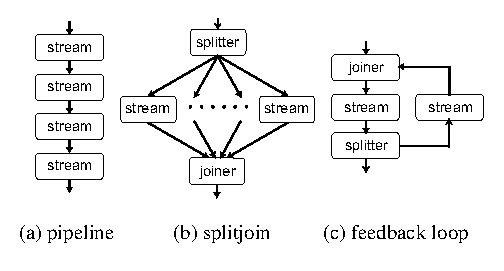
\includegraphics[scale=1, angle=0]{./constructs-eg.eps}
%}
% \vspace{-6pt}
% \nocaptionrule
 \caption{Hierarchical streams in StreamIt.}
 \label{fig:containers}
\end{center}
\end{figure}

\begin{figure}[t]
\begin{center}
\vspace{-12pt}
% \framebox{
 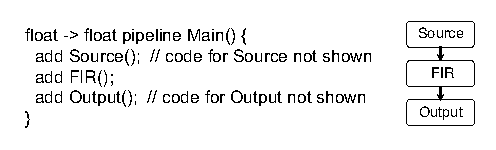
\includegraphics[scale=1, angle=0]{./pipeline-eg.eps}
%}
% \vspace{-6pt}
% \nocaptionrule
 \caption{Example pipeline with FIR filter.}
 \label{fig:pipeline}
%\vspace{-18pt}
\end{center}
\end{figure}

In StreamIt, the
application developer focuses on the hierarchical assembly of the
stream graph and its communication topology, rather than on the 
explicit management of the data buffers between filters.
StreamIt provides three hierarchical structures for composing filters
into larger stream graphs (see Figure~\ref{fig:containers}). The 
{\it pipeline} construct composes streams in sequence, with the output
of one connected to the input of the next.   An example of a pipeline
appears in Figure~\ref{fig:pipeline}.

The {\it splitjoin} construct distributes data to a set of parallel
streams, which are then joined together in a round robin fashion.  In
a splitjoin, the {\it splitter} performs the data scattering, and the
{\it joiner} performs the gathering. A splitter is a specialized
filter with a single input and  multiple output channels. On 
every execution step, it can distribute its output to any one of
its children in either a {\it duplicate} or a {\it roundrobin}
manner. For the former, incoming data are replicated to every
sibling connected to the splitter. For the latter, data are scattered
in a round robin manner, with each item sent to exactly one child
stream, in order.  The splitter type and the weights for distributing data to
child streams are declared as part of the syntax (e.g., \texttt{split
duplicate} or \texttt{split roundrobin($w_1,\ldots,w_n$)}). The
splitter counterpart is the joiner. It is a specialized filter with  
multiple input channels but only one output channel. The joiner
gathers data from its predecessors in a round robin manner (declared
as part of the syntax) to produce a single output stream.

StreamIt also provides a {\it feedback loop} construct for introducing
cycles in the graph.

%\section{Execution Model}
%\label{sec:execmodel}

%% A StreamIt program is represented by a hierarchical graph,
%% where the leaf nodes are filters, splitters, and joiners, and
%% the composite nodes are pipelines, splitjoins, and
%% feedback-loops. Edges in the graph represent data channels, which 
%% operate as FIFO queues.
\paragraph*{Execution Model}
As noted earlier, an actor (i.e., a filter, splitter, or joiner)
executes whenever there are enough data items on its input 
tape. In StreamIt, actors have  two epochs
of execution: one for initialization, and one for the {\it steady
state}. The initialization primes the input tapes to allow filters with
peeking to execute the very first instance of their work functions.
%%initialization in this setting is similar to the prologue stage in
%%software pipelining. 
A steady state is an execution that does not change the
buffering in the channels: the number of items on each channel
after the execution is the same as it was before the execution. 
Every valid stream graph has a steady state~\cite{LM87-i}, and within
a steady state, there are often many possibilities for interleaving
actor executions. 
%% The steady state schedule has the property that
%% the amount of data buffered between any two actors does not change
%% before and after the actor executions.
\begin{figure}[t]
\begin{center}
%%\vspace{-24pt}
%\vspace{24pt}
 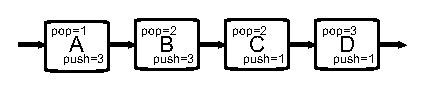
\includegraphics[scale=1, angle=0]{./pipe-with-rates.eps}
%\vspace{-6pt}
% \nocaptionrule
 \caption{Example pipeline.}
 \label{fig:pipe-with-rates}
\end{center}
%\vspace{-12pt}
\end{figure}
An example of a steady state for the pipeline in
Figure~\ref{fig:pipe-with-rates} requires filter \texttt{A} to fire
4 times, \texttt{B} 6 times, \texttt{C} 9 times, and
\texttt{D} 3 times. 
% Because in StreamIt the filters are
% independent (i.e., they do not share state), they can execute
% concurently. In a uniprocessor setting (which is what we use for our
% evaluation), we can only run one filter at time. Therefore, 
% The data generated by one actor are buffered (cached) until they are
% consumed.

\paragraph*{Compilation Process}
The StreamIt compiler derives the initialization and steady state
schedules~\cite{karczma-lctes03} and outputs a C program that includes
the initialization and work functions, as well as a driver to execute
each of the two schedules. Our compilation process allows the StreamIt
compiler to focus on high level optimizations, and relies on existing
compilers to perform machine-specific optimizations such as register
allocation, instruction scheduling, and 
code generation---this two step approach affords us a
great deal of portability (e.g., code generated from the StreamIt
compiler is compiled and run on three different machines as reported
in Section~\ref{sec:evaluation}).

%% For example, referring to
%% Figure~\ref{fig:pipe-with-rates}, the compiler generates the following
%% sample code for running the steady state schedule:
%% %\begin{scriptsize}
%% \begin{verbatim}
%% run_steady_state() {
%%   for (i = 0; i < 4; i++) A_work();
%%   for (i = 0; i < 6; i++) B_work();
%%   for (i = 0; i < 9; i++) C_work();
%%   for (i = 0; i < 3; i++) D_work();
%% }
%% \end{verbatim}
%% %\end{scriptsize}
%% To execute the program, the steady state is wrapped with
%% another loop that invokes the steady state a designated number of
%% times. Preceding the state steady, a similar initialization schedule
%% is run to prime the data buffers.
%, and following the steady state, an
%epilogue is run to drain the buffers as necessary.

%% \begin{figure}[t]
%% \begin{center}
%% \vspace{-12pt}
%%  \psfig{figure=ssi.eps,width=3in}
%%  \vspace{-6pt}
%%  \caption{Instruction size (in bytes along the y-axis) per filter
%%  (x-axis) occurring in a steady state execution of FFT.}
%%  \label{fig:ssi-single}
%% \vspace{-18pt}
%% \end{center}
%% \end{figure}

\section{Model of Computation}
\label{model}

The model of computation employed for this paper is a general model
that is agnostic of input language.  The semantics of the model are
built upon synchronous dataflow (SDF)~\cite{leeSDF}.  Although
inspired by the StreamIt programming language, the model can represent
aspects of other streaming languages such as Brook~\cite{brook04},
Lime~\cite{lime10}, SPL~\cite{spl09} and SPUR~\cite{spur05samos}.
Consider a directed graph $G = (V, E)$ corresponding to a streaming
application. $F \in V$ is a filter in the application and $(f, g) \in
E$ is an edge (or {\it channel}) in the graph that denotes
communication from $f$ to $g$ using a FIFO channel.  Each filter is
described by rate declarations, data reorganization patterns,
and compute functions as described below. The techniques in this paper
require static-rate graphs, i.e., all of the quantities of the filters
are statically determinable.

%  Figure~\ref{fig:streamgraph} gives an example
% stream graph for a FM radio with an equalizer.  The figure also
% includes details for two of the filters; the details are explained
% below.

% The filter is the basic unit of execution in our model.  Each filter
% is described by multiple rate declarations, data reorganization
% patterns, and compute functions.  Basically, each filter defines the
% number of items it consumers and produces each time it is executed.
% The execution of a stream graph is represented by a {\it schedule} of
% a graph $G$.  A schedule gives a multiplicity for each filter $F \in
% V$ that denotes how many times to fire filter $F$.  When a schedule is
% executed, each filter fires when it has buffered enough input to
% satisfy its input requirement (a filter will not fire more times than
% given by a schedule).  In our notation, a schedule is represented by
% the variable $\Sigma$, and it denotes a mapping from filters to
% non-negative integers. The multiplicity of filter $F$ in schedule
% $\Sigma$ is denoted by $M(\Sigma, F)$.

For each filter, $F \in V$, a {\it work} function, $W_F$, is defined.
The work function defines the atomic execution step for each filter.
For each filter, $F \in V$, a {\it prework} function, $W_F^P$, can
also be defined.  Prework describes a computation step that executes
once at the first firing of a filter.  The prework function is
executed only once per execution of the {\it application}; it
describes any special initialization behavior required for a
filter. We denote a function with the variable $\mathcal{F} \in \{W^p,
W\}$.  We sometimes leave out the subscript that denotes the filter if
it is clear which work or prework function is intended.

For each filter $F \in V$ we define the following:
\begin{itemize}

\item $o(\mathcal{F}, F)$, or {\it pop} rate, is the number of items
  dequeued from $F$'s input buffer per firing of $\mathcal{F}$.

\item $e(\mathcal{F}, F)$, or  {\it peek} rate, 1 $+$ the greatest index that is read (but
  not necessarily dequeued) from $F$'s input buffer per firing of
  $\mathcal{F}$. 

\item $u(\mathcal{F}, F)$, or {\it push} rate , the number of items enqueued to $F$'s
output buffer per firing of $\mathcal{F}$.  

\end{itemize}

\noindent Sliding window filters have a peek rate greater than the pop
rate.  We somethings refer to sliding window filters as {\it peeking}
filters. Figure~\ref{fig:pipeline-example}(a)
demonstrates a peeking filter.  The figures shows that the window of
items read for 3 consecutive firings of the filter overlap.  For the
work function execution, a peeking filter $F$ requires $e(W_F, F)$
items to be on its input channel(s) to fire.  $F$ will consume
(dequeue) the first $o(W_F, F)$ items after the firing of the work function.

\begin{figure}[t]
\centering
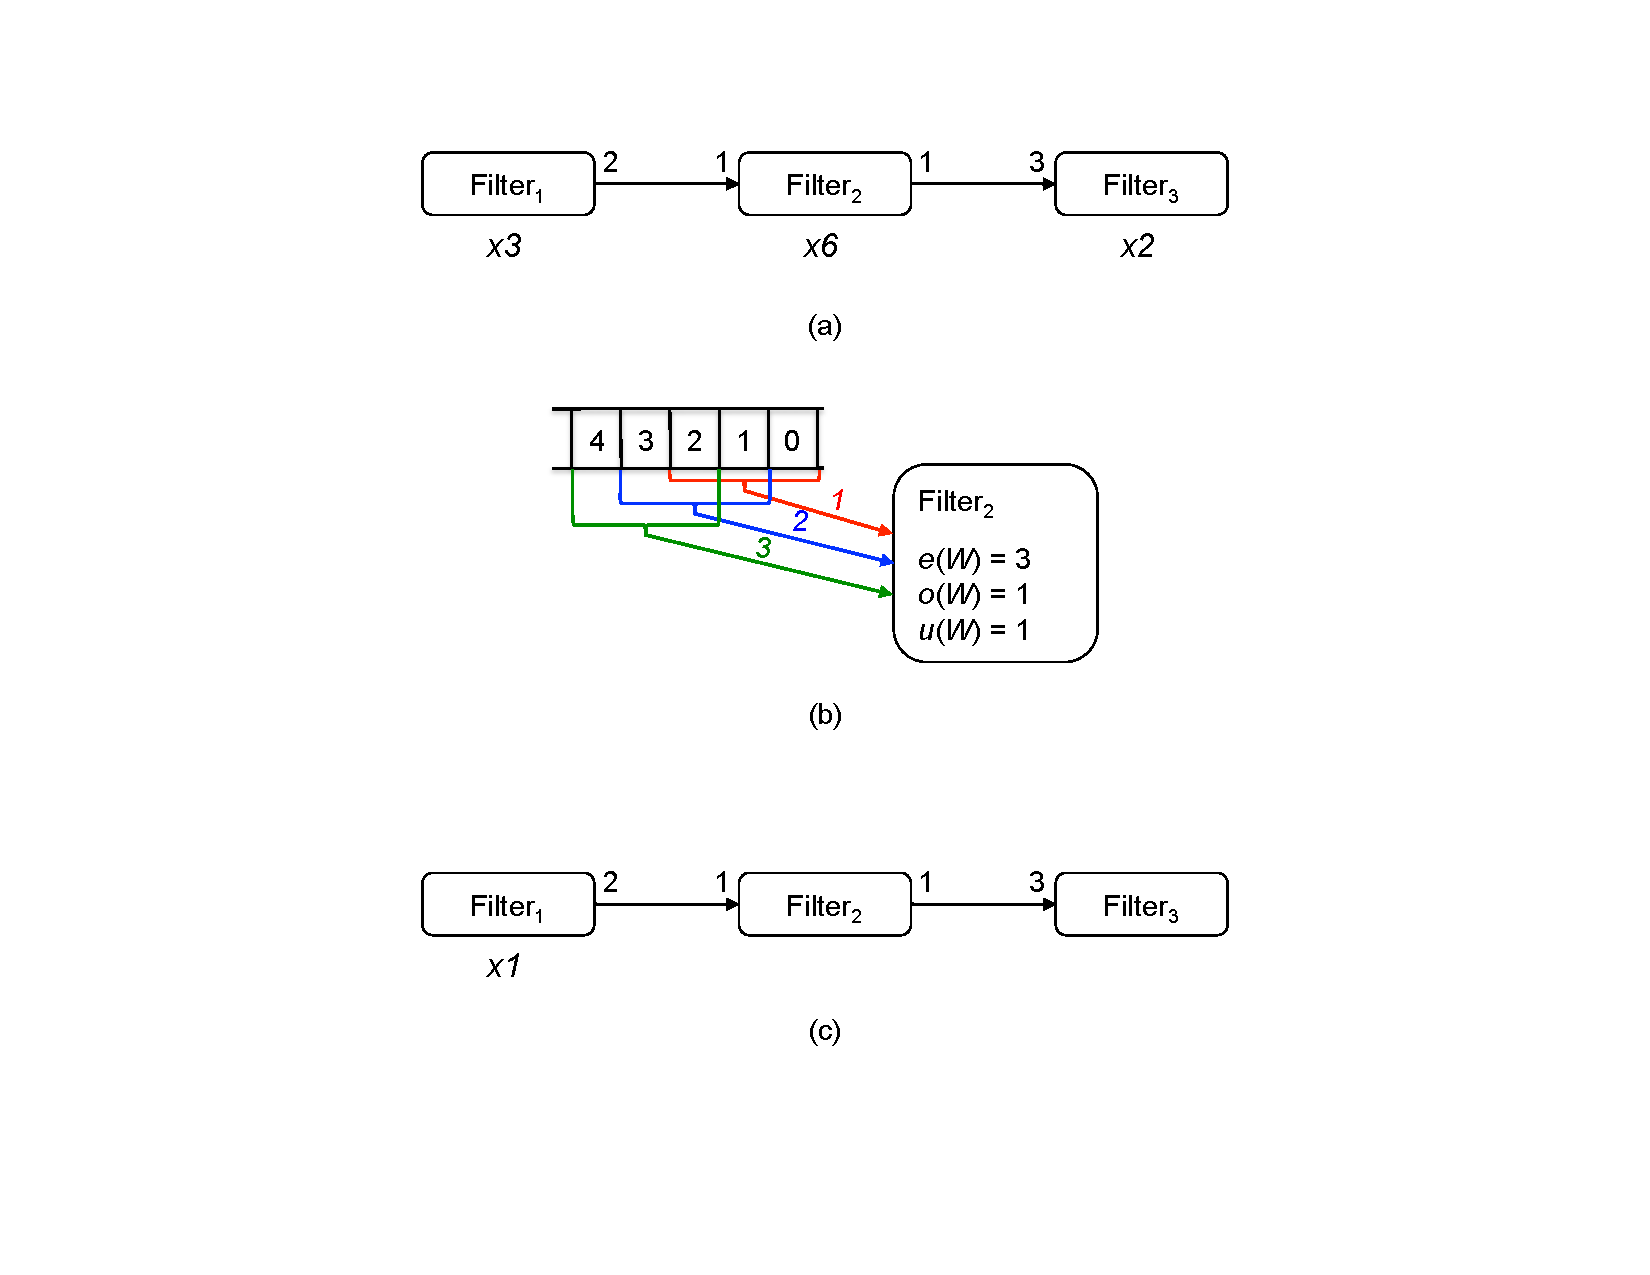
\includegraphics[width=3.0in]{figures/pipeline-example.pdf}
\caption[A pipeline of three filters with schedules.]{ (a) gives
  details for a sliding window filter.  The figure
  shows the window of items read for 3 consecutive firings of the
  filter.  Notice the overlapping in the windows.  (b) presents a pipeline of
  three filters with push and pop rates.  (b) also gives a
  legal steady-state schedule and initialization schedule for the
  three filters. $C(\mt{Filter}_2) = 2$ and
$C(\mt{Filter}_1) = C(\mt{Filter}_3) = 0$. 
  \label{fig:pipeline-example}}
\vspace{-10pt}
\end{figure}

A schedule gives a multiplicity for each filter $F \in V$ that denotes
how many times to fire filter $F$. A {\it steady-state schedule} can
be calculated such that all filters fire in the schedule, and the
schedule can be repeated indefinitely~\cite{lee87}.  Steady-state
execution of the graph entails repeating the steady-state schedule for
as much input as is expected.  Execution of the stream graph is
conceptually wrapped in an outer loop that continuously executes the
steady-state schedule.  Figure~\ref{fig:pipeline-example}(b) gives an
example of a steady-state schedule calculated for a graph that
consists of three filters in a pipeline.  All the multiplicities of
the steady-state can be multiplied by the same constant $c$, and the
result will still be a valid steady-state.  We call this process {\it
  increasing} the steady-state of the graph by $c$.

Our model does not deal with arbitrary schedules of filter executions.
The steady-state schedule, $S$, is explicitly represented.
Furthermore, an {\it initialization} schedule, $I$, is explicitly
represented that enables the steady-state schedule in the presence of
peeking filters.  An initialization schedule is required if peeking is
present in a graph to enable the calculation and execution of a
steady-state schedule~\cite{karczmarek-lctes03}.  After the initialization
schedule executes, each filter $F$ is guaranteed to have at least
$e(W_F, F) - o(W_F, F)$ items in its input buffer.
Figure~\ref{fig:pipeline-example}(b) gives a legal initialization
schedule for the pipeline that enables the peeking in filter
$\mt{Filter}_2$.  During application execution, the initialization
schedule is executed once followed by an infinite repetition of the
steady-state schedule.  The number of items remaining on $F$'s input
channel(s) after execution of the initialization schedule is
represented by $C(F)$.

In our notation, a schedule is represented by the variable $\Sigma$,
and it denotes a mapping from filters to non-negative integers. In our
execution model, only an initialization schedule and a steady-state
schedule are considered (thus $\Sigma \in I,S$). The
multiplicity of filter $F$ in schedule $\Sigma$ is denoted by
$M(\Sigma, F)$.  

A filter may have multiple incoming edges and/or multiple outgoing
edges.  Filter inputs are organized into a single internal FIFO buffer for the
filter to read according to an {\it input distribution pattern}, and
filter outputs are distributed from a single internal output FIFO
buffer according to an {\it output distribution pattern}.   
The input distribution pattern is represented as:
{\ninepoint
\[ \mt{ID}(\Sigma, F) \in (\mathbb{N} \times E)^n = ((w_1,e_1), (w_2,
e_2), ..., (w_n, e_n))\]
}
\noindent Where $n$ is the width of the input distribution pattern.
The input distribution describes the round robin joining pattern for
organizing the input data into the filter's single internal FIFO
buffer, where $w_i$ items are received from edge $e_i$ before
proceeded to the next edge, $e_{i+i}$.

The output distribution pattern describes both round-robin
splitting and duplication in a single structure:
{\ninepoint
\[ \mt{OD}(\Sigma, F) \in (\mathbb{N} \times (P(E)-\emptyset))^m = ((w_1,d_1), (w_2,
d_2), ..., (w_n, d_n))\]
}
\noindent Where $P(E)$ is the powerset of $E$.  Each $d_i$ is called
the {\it dupset} of weight $i$.  The dupset $d_i$ specifies that $w_i$
items be duplicated to the edges of the dupset.  Each tuple denotes
that $w_i$ output items of $F$ are duplicated to the edges of $d_i$
before moving on to the next tuple.

\begin{figure}[t]
\centering
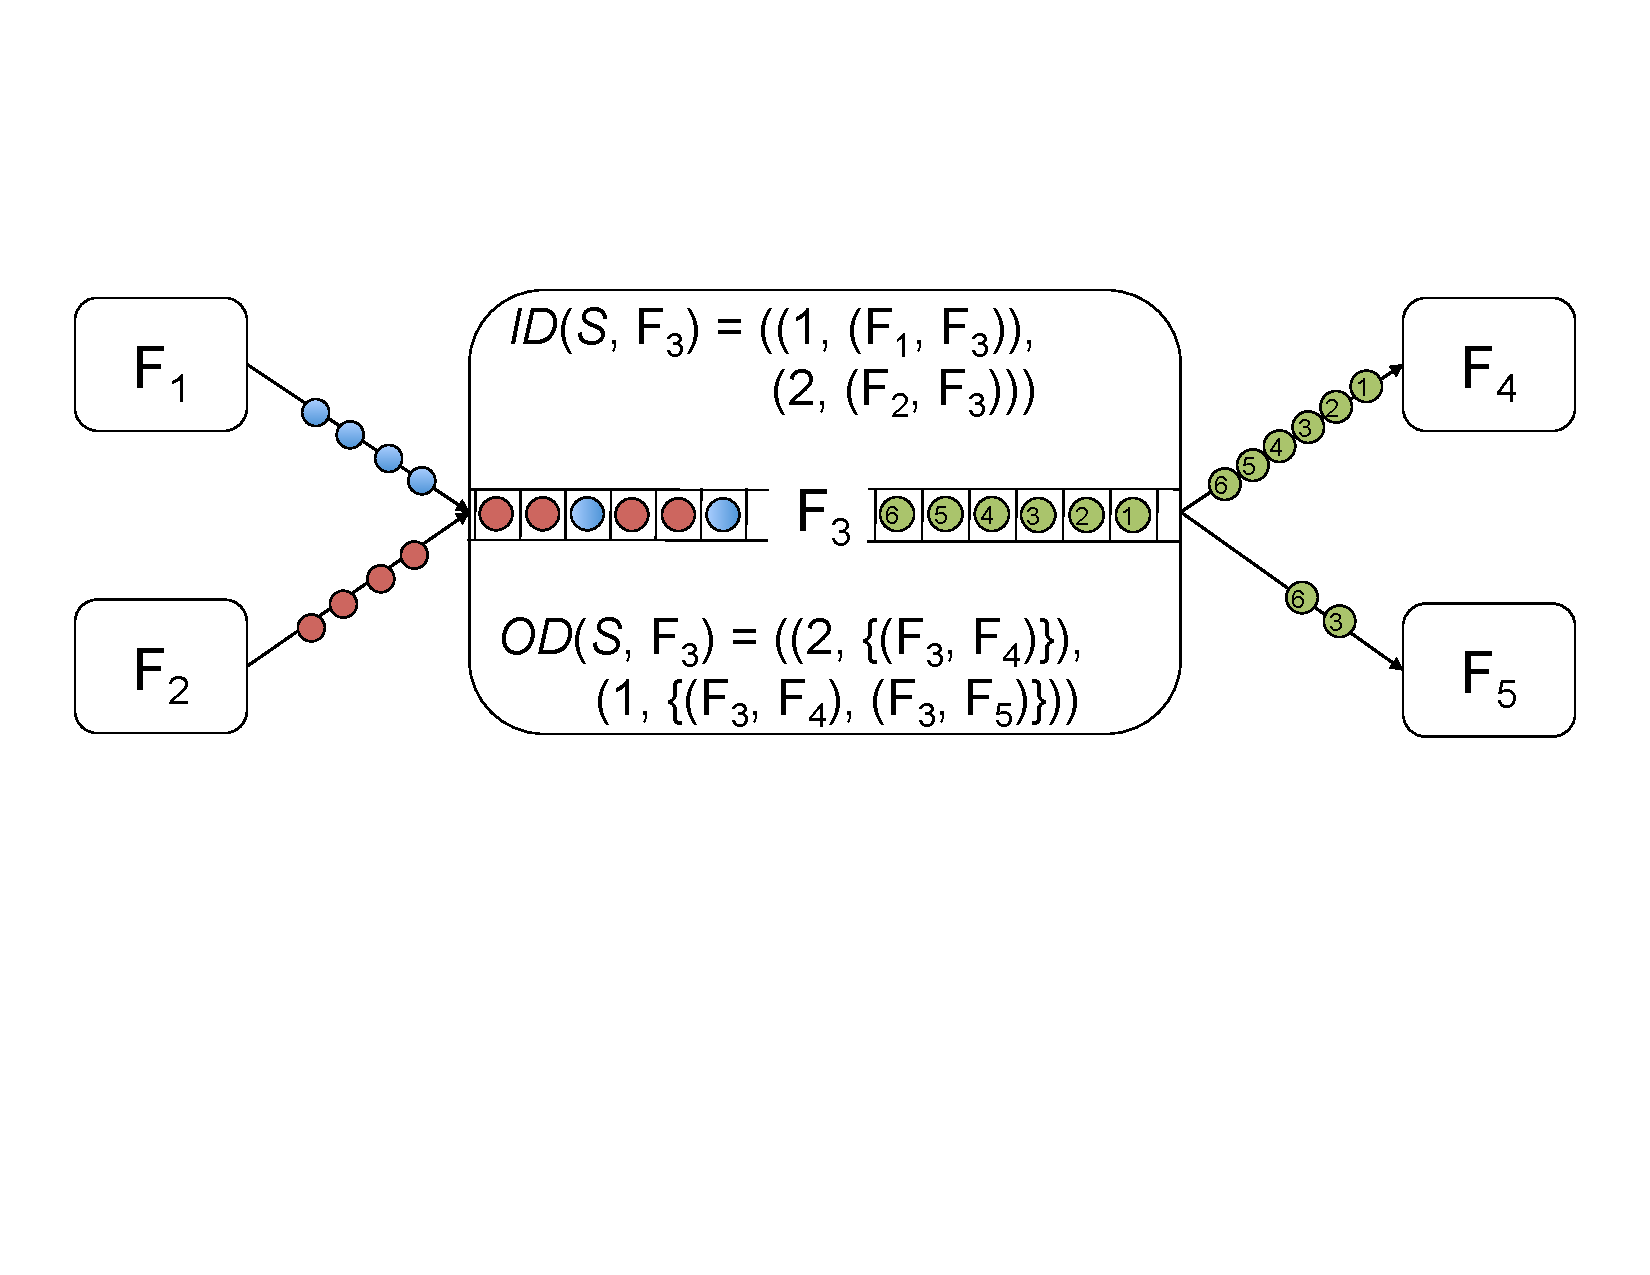
\includegraphics[width=3in]{figures/dist-example.pdf}
\caption[Example of input and output distribution.]{
An example of a filter with non-trivial input and output distribution patterns.
Filter $F_3$ has both multiple inputs and multiple outputs.  The input
items from the multiple inputs are joined in the pattern described by
its input distribution ($ID$): receive 1 item from $F_1$ and 2
items from $F_2$, and repeat.  $F_3$'s output items are distributed to
its multiple outputs as described by the output distribution pattern
($OD$):  2 items to $F_4$, then 1 item is duplicated to both $F_4$ and
$F_5$.  The output items of $F_3$ are indexed to show how they are
distributed to $F_4$ and $F_5$.
\label{fig:dist-example}}
\vspace{-10pt}
\end{figure}

The input and output distributions are repeated as needed for the
schedule that is being executed.  The start of each steady-state
iteration resets the input and output distributions to the first tuple.
Figure~\ref{fig:dist-example} highlights an example of a filter with
both multiple inputs and multiple outputs, and how the distribution
patterns translate into scattering and gathering.

Let $\mt{RO}(F_1, F_2, \Sigma)$ be the ratio of output items $F_1$
splits along the edge $(F_1, F_2)$ to the total number of items that
$F_1$ produces in the schedule $\Sigma$.  This can be calculated from
$F_1$'s output distribution pattern for $\Sigma$.  For example, in
Figure~\ref{fig:dist-example}, $\mt{RO}(F_3, F_4) = 1$ and
$\mt{RO}(F_3, F_5) = \frac{1}{3}$.  Conversely, let $\mt{RI}(F_1, F_2,
\Sigma)$ be the percentage of total input items that $F_2$ receives
from $F_1$ for $\Sigma$.  For example, in
Figure~\ref{fig:dist-example}, $\mt{RI}(F_2,F_3) = \frac{2}{3}$.

% Let $s(\mathcal{F}, F)$ denote the execution time (in cycles, with
% respect to a given real or conceptual machine) of function
% $\mathcal{F}$ of filter $F$.  For many of the static scheduling
% techniques covered in this thesis, we calculate a static estimation of
% the total amount of work for a filter $F$ in the steady-state, $s(W,
% F) \cdot M(S, F)$.  We often use the term {\it work estimation} to
% denote this quantity.

\mysection{Optimizations}
\label{sec:optimization}

We consider two types of optimizations.  The first is to remove
redundant state variables from the linear state space representation.
This reduces the memory allocation for a program as well as the number
of loads and stores, which are typically slow and power-hungry
operations. It also eliminates computations that involve the removed
states.  The second optimization is to reduce the parametrization of a
state space representation by refactoring the matrices to contain more
zero and one entries.  This directly eliminates computations, as the
compiler statically evaluates $0 \cdot x = 0$ and $1 \cdot x = x$
rather than performing the multiplications at runtime.  Both the state
removal optimization and parameter reduction optimization are
formulated as a series of general transformations on the underlying
state space representation.

\mysubsection{State Space Transformations}

For any state space equation pair, there are an infinite number of
transformations to an equivalent state space system.  These
transformations involve a change of basis of the state vector
$\vec{\mathbf{x}}$ to $\mathbf{T} \vec{\mathbf{x}}$, where
$\mathbf{T}$ is an invertible matrix. Consider the state update
equation $\vec{\dot{\mathbf{x}}} = \mathbf{A} \vec{\mathbf{x}} +
\mathbf{B} \vec{\mathbf{u}}$. Multiplying the entire equation by
$\mathbf{T}$ yields:
\starteqnstar
\mathbf{T} \vec{\dot{\mathbf{x}}} = \mathbf{TA} \vec{\mathbf{x}} +
\mathbf{TB} \vec{\mathbf{u}}
\doneeqnstar
Since $\mathbf{T}^{-1} \mathbf{T} = \mathbf{I}$, we can write:
\starteqnstar
\mathbf{T} \vec{\dot{\mathbf{x}}} & = & \mathbf{TA}
(\mathbf{T}^{-1} \mathbf{T}) \vec{\mathbf{x}} + \mathbf{TB}
\vec{\mathbf{u}} ~~=~~ \mathbf{TA}
\mathbf{T}^{-1} (\mathbf{T} \vec{\mathbf{x}}) + \mathbf{TB} \vec{\mathbf{u}} \\
\vec{\mathbf{y}} & = & \mathbf{C} (\mathbf{T}^{-1} \mathbf{T})
\vec{\mathbf{x}} + \mathbf{D} \vec{\mathbf{u}} ~~~~~\hspace{1.1pt}~=~~ \mathbf{C}
\mathbf{T}^{-1} (\mathbf{T} \vec{\mathbf{x}}) + \mathbf{D}
\vec{\mathbf{u}}
\doneeqnstar
where we have introduced the output equation as well. Let
$\vec{\mathbf{z}} = \mathbf{T} \vec{\mathbf{x}}$.
$\vec{\mathbf{z}}$ is a new state vector related to the old state
vector $\vec{\mathbf{x}}$ by the change of basis $\mathbf{T}$.
Substituting into the above equations yields:
\starteqnstar
\vec{\dot{\mathbf{z}}} & = & \mathbf{TA} \mathbf{T}^{-1} \vec{\mathbf{z}} + \mathbf{TB} \vec{\mathbf{u}} \\
\vec{\mathbf{y}} & = & \mathbf{C} \mathbf{T}^{-1}\vec{\mathbf{z}}
+ \mathbf{D}\vec{\mathbf{u}}
\doneeqnstar

This is precisely the original state space equation pair,
with $\mathbf{A}$, $\mathbf{B}$, and $\mathbf{C}$ transformed to
$\mathbf{T} \mathbf{A} \mathbf{T}^{-1}$, $\mathbf{T} \mathbf{B}$,
and $\mathbf{C} \mathbf{T}^{-1}$, respectively.

For a StreamIt state space representation $\cal{R}$, we must determine
how the other values change.  Since the old state vector
$\vec{\mathbf{x}}$ is multiplied by $\mathbf{T}$, the old initial
state vector is multiplied by $\mathbf{T}$.  The initialization update
equation is analogous to the standard update equation, so
$\mathbf{B_{pre}}$ is transformed to $\mathbf{T} \mathbf{B_{pre}}$.  The
number of states, inputs, and outputs is the same, so $s$, $o$, and
$u$ are unchanged.

\mysubsection{State Removal}
\label{sec:state-removal}

There are two types of states that can be removed from a state space
system without changing its behavior: unreachable and unobservable
states.  Informally, unreachable states are unaffected by inputs and
unobservable states have no effect on outputs.  If there are two
redundant states in a filter, then both may reachable and observable
as the program is written.  However, following a series of
transformations, one of the redundant states can be converted to an
unreachable or unobservable state, allowing it to be removed.

More formally, the $i$th state is reachable if and only if at least
one of the following is true:
\begin{enumerate}
\item \parbox[t]{2.8in}{The state is initialized to a non-zero value.
That is, the $i$th entry of $\overrightarrow{\mathbf{initVec}}$ is
non-zero or $\exists j~\mbox{s.t.}~\mathbf{B_{pre}}[i,j] \ne 0$.}

\item \parbox[t]{2.8in}{The state directly depends on an input.  That
is, $\exists j~\mbox{s.t.}~\mathbf{B}[i,j] \ne 0$.}

\item \parbox[t]{2.8in}{The state directly depends on another
reachable state.  That is, $\exists j \ne
i~\mbox{s.t.}~\mathbf{A}[i,j] \ne 0$ and $j$ is a reachable state.}
\end{enumerate}
All states in the system are either reachable or unreachable.
Unreachable states always have a value of zero, as they are
initialized to zero and are never updated by a non-zero value (i.e.,
by a reachable state or an input).  Therefore, unreachable states can
be removed from the state space representation, since they have no
effect on any other states or output values.

The $i$th state is observable if and only if at least one of the
following is true:
\begin{enumerate}
\item \parbox[t]{2.8in}{An output directly depends on the state.  That
is, $\exists j~\mbox{s.t.}~\mathbf{C}[j,i] \ne 0$.}

\item \parbox[t]{2.8in}{Another observable state directly depends on
the state.  That is, $\exists j \ne i~\mbox{s.t.}~\mathbf{A}[j,i] \ne
0$ and $j$ is an observable state.}
\end{enumerate}
All states in the system are either observable or unobservable.  The
unobservable states are not used to update the observable states and
are not used to determine the outputs.  Therefore, all unobservable
states can be removed from a representation (regardless of their
initial values).

There is a simple algorithm to refactor the states of a system and
expose the unreachable and unobservable states~\cite{Mayne}.  For
unreachable states, the algorithm assumes that there is no
initialization stage, i.e., that $\overrightarrow{\mathbf{initVec}}$
and $\mathbf{B_{pre}}$ are zero.  We first describe the basic
algorithm and then extend it to handle the initialization stage.

To detect unreachable states, the algorithm performs row
operations\footnote{\smaller Performing a row operation operation on a
matrix is equivalent to left-multiplying it by some invertible matrix,
while performing a column operation is equivalent to right-multiplying
by some invertible matrix.} on the augmented matrix $\left [
\begin{array} {cc} \mathbf{A} & \mathbf{B} \end{array} \right ]$.  To 
maintain the proper input/output relationship of the system,
corresponding inverse column operations are performed on $\mathbf{A}$
and $\mathbf{C}$.  The row operations achieve a special type of
row-echelon form.  In this form, the last non-zero entry in each row
is a 1 (called the ending 1) and the ending 1 in a given row is to the
left of the ending 1 in lower rows.  Once the augmented matrix is in
the desired form, row $i$ represents an unreachable state if there are
no non-zero entries past the $i$th column.  This naturally expresses
the constraint that the $i$th state does not depend on any input
(columns of $\mathbf{B}$) or on any possibly reachable state (later
columns of $\mathbf{A}$).  In the absence of an initialization stage,
all unreachable states identified in this way can be removed from the
system.

For unobservable states, the same procedure is applied to the
augmented matrix $\left [\begin{array} {cc} \mathbf{A}^T &
\mathbf{C}^T \end{array} \right ]$.  In the echelon form, row $i$
represents an unobservable state if there are no non-zero entries past
the $i$th column.  Intuitively, the rows of the transposed matrices
represent how a given state is used, rather than how it is calculated.
The identified states are unobservable because they are used neither
in the calculation of an output (columns of $\mathbf{C}^T$) nor in
possibly observable states (later columns of $\mathbf{A}^T$).  All of
these unobservable states can be safely removed from the system (even
if they are assigned an initial value).

\looseness+1 To handle the initialization stage for unreachable
states, a minor extension is needed.  If a state is assigned a
non-zero value during initialization, either as a constant (a non-zero
entry in $\overrightarrow{\mathbf{initVec}}$) or from the input (a
non-zero entry in $\mathbf{B_{pre}}$), the state must be considered
reachable.  Further, any dependent states must also be considered
reachable.  This classification can easily be performed as a
post-processing step on the set of candidate unreachable states
identified by the algorithm above.  If any candidate is initialized to
a non-zero value or directly depends (via the $\mathbf{A}$ matrix) on
a state outside the set, then the candidate is removed from the set.
When no further candidate can be removed from the set, the set
contains nothing but genuine unreachable states.

%% The general algorithm for identifying unreachable states works as
%% follows.  First, it uses the previous algorithm~\cite{Mayne} to
%% identify {\it candidate} unreachable states.  Suppose that there are
%% $k$ candidates.  The candidate states are moved to the top of the
%% state vector via a series of row operations.  Following this
%% reordering, the sub-matrix $\mathbf{A}[1:k;1:k]$ represents the
%% dependences between candidate unreachable states.  As detailed below,
%% this sub-matrix is converted to an upper-triangular form (i.e., all
%% entries below the diagonal are zero) while maintaining the
%% input/output relationship of the system.  Finally, the candidate
%% states are considered in reverse order (from $k$ to $1$).  The $i$th
%% state is declared reachable if at least one of the following is true:
%% \begin{itemize}
%% \item The $i$th state is initialized to a non-zero value.

%% \item The $i$th state directly depends on another reachable state.
%% \end{itemize}

%%%%%%%%%%%%%%%%%%%%%%%%%%%%%%%%%%%%%%%%%%%%%%%%%%%%%%%%%

\mysubsubsection{Expanding the Scope}

So far we have considered optimizations that affect $\mathbf{A}$,
$\mathbf{B}$, and $\mathbf{C}$. Since the optimizations are entirely
the result of state transformations, they do not affect $\mathbf{D}$,
which is independent of the choice of state space basis.  However, if
all of the inputs are stored as states, then all of the entries of
$\mathbf{D}$ are moved into $\mathbf{A}$ and can then be changed by
state optimizations.

We have already discussed how to store inputs as states. When every
input is stored as a state, the new state-equation pair is:
\vspace{2pt}
\starteqnstar
\left [ \begin{array} {c} \vec{\dot{\mathbf{x}}} \\
\vec{\dot{\mathbf{x_{in}}}} \end{array} \right ] & = & \left [
\begin{array} {cc} \mathbf{A} & \mathbf{B} \\ \mathbf{0} &
\mathbf{0} \end{array} \right ] \left [ \begin{array} {c}
\vec{\mathbf{x}} \\ \vec{\mathbf{x}}_{{\mathbf{in}}} \end{array} \right ]
+ \left [ \begin{array} {c} \mathbf{0} \\ \mathbf{I} \end{array}
\right ] \vec{\mathbf{u}} \vspace{1pt} \\
\vec{\mathbf{y}} & = & \left [ \begin{array} {cc} \mathbf{C} &
\mathbf{D} \end{array} \right ] \left [ \begin{array} {c}
\vec{\mathbf{x}} \\ \vec{\mathbf{x}}_{{\mathbf{in}}} \end{array} \right ]
+ \mathbf{0} \vec{\mathbf{u}}
\doneeqnstar
\vspace{2pt}
These states should be added before state removal is performed. It may
seem counter-intuitive that we first add states, then seek to remove
them. However, the added states represent computations involving
$\mathbf{D}$ which were not considered before. Removing some of these
states can result in reducing computations involving $\mathbf{D}$.

\mysubsection{Parameter Reduction}
\label{sec:parameter-reduction}

After removing as many states as possible, additional computations can
be eliminated by transforming the state space system to one with fewer
non-zero, non-one entries (termed parameters). If $\mathbf{A}$,
$\mathbf{B}$, and $\mathbf{C}$ are completely filled, there are
$s*(s+o+u)$ parameters. Ackermann and Bucy \cite{Ackermann/Bucy} show
a general form in which $\mathbf{A}$ and $\mathbf{C}$ have at most
$s*(o+u)$ parameters ($\mathbf{B}$ may contain any number of
parameters), assuming there are no unobservable or unreachable
states. They derive this form using system impulse responses. We
achieve the same form using row operations on the augmented matrix
$\left [ \begin{array} {cc} \mathbf{A}^T & \mathbf{C}^T \end{array} \right ]$. 
The desired form is:

\newpage
~ \\ \vspace{-24pt}
\starteqnstar
\mathbf{A}^T &=& \left [ \begin{array} {ccccc} \mathbf{L_1} &
\mathbf{A_{12}} & \mathbf{A_{13}} & ... & \mathbf{A_{1u}} \\
\mathbf{0} & \mathbf{L_2} & \mathbf{A_{23}} & ... &
\mathbf{A_{2u}} \\ \mathbf{0} & \mathbf{0} & \mathbf{L_3} & ... &
\mathbf{A_{3u}} \\ ... & ... & ... & ... & ... \\ \mathbf{0} &
\mathbf{0} & \mathbf{0} & ... & \mathbf{L_u} \end{array} \right ] \\ ~ \\
\mathbf{C}^T &=& \left [ \begin{array} {ccccc} 1 & 0 & 0 & ... &
0 \\ 0 & 0 & 0 & ... & 0 \\ ... & ... & ... & ... & ... \\ 0 & 1 &
0 & ... & 0 \\ 0 & 0 & 0 & 0 & 0 \\ ... & ... & ... & ... & ... \\
0 & 0 & 0 & ... & 1 \end{array} \right ]
\doneeqnstar

The matrices $\mathbf{A_{ij}}$ are rectangular, and the matrices
$\mathbf{L_i}$ are square, but do not necessarily have the same
dimensions as each other. These matrices have the form:
\starteqnstar
~~\mathbf{A_{ij}} = \left [ \begin{array} {cccc} \hspace{-1pt}0 & 0 & ... & *
\hspace{-1pt}\\\hspace{-1pt} ... & ... & ... & ... \hspace{-1pt}\\\hspace{-1pt} 0 & 0 & ... & *\hspace{-1pt} \end{array} \right ] ~~
\mathbf{L_i} = \left [ \begin{array} {ccccc} \hspace{-1pt}0 & 0 & ...
& 0 & * \hspace{-1pt}\\\hspace{-1pt} 1 & 0 & ... & 0 & * \hspace{-1pt}\\\hspace{-1pt} 0 & 1 & ... & 0 & * \hspace{-1pt}\\\hspace{-1pt}
... & ... & ... & ... & ... \hspace{-1pt}\\\hspace{-1pt} 0 & 0 & ... & 1 & *\hspace{-1pt} \end{array}
\right ]
\doneeqnstar

The entries marked with a * are the parameters of the system.  This is
known as the observable canonical form of the system. In contrast, the
reachable canonical form defines $\mathbf{A}$ and $\mathbf{B}$ instead
of $\mathbf{A}^T$ and $\mathbf{C}^T$ (there may be any number of
parameters in $\mathbf{C}$ rather than $\mathbf{B}$).

Figure~\ref{fig:param} gives pseudocode for a simple algorithm to
attain the form above.  The pseudocode does not include the
corresponding inverse column operations that must go with all row
operations.

It is possible that one type of form has fewer parameters than the
other. Thus, we perform the above algorithm on $\left [
\begin{array} {cc} \mathbf{A}^T & \mathbf{C}^T
\end{array} \right ]$ as noted to produce the observable form, as well as on $\left [
\begin{array} {cc} \mathbf{A} & \mathbf{B} \end{array} \right
]$ to produce the reachable form.  We compare the forms and use the
one with fewest parameters.

\mysubsubsection{Staged Execution}

Using input state variables corresponds to executing a state space
block in two stages:
\begin{enumerate}
\vspace{\itemshrink} \item Put inputs into input state variables.

\vspace{\itemshrink} \item Execute the original block, using input states instead of
actual inputs.
\vspace{\itemshrink} \end{enumerate}

We can add additional stages by having multiple sets of input
states---$\vec{\mathbf{x}}_{{\mathbf{in1}}}$,
$\vec{\mathbf{x}}_{{\mathbf{in2}}}$, etc.  After each execution, the
first set is moved to the second set, the second set is moved to the
third set, and so on.  Suppose there are $k$ input sets. We can write
the state space equation pair as follows: \starteqnstar \left
[\hspace{-1.4pt}
\begin{array} {c} \vec{\dot{\mathbf{x}}} \\
\vec{\dot{\mathbf{x}}}_{{{\mathbf{ink}}}} \\ ... \\
\vec{\dot{\mathbf{x}}}_{{{\mathbf{in2}}}} \\
\vec{\dot{\mathbf{x}}}_{{{\mathbf{in1}}}}
\end{array} \hspace{-1.4pt} \right] &\hspace{-6pt}=\hspace{-6pt}& \left [\hspace{-1.4pt} \begin{array} {ccccc}
\mathbf{A} & \mathbf{B} & \mathbf{0} & ... &
\mathbf{0} \\ \mathbf{0} & \mathbf{0} & \mathbf{I} & ... & \mathbf{0} \\
... & ... & ... & ... & ... \\ \mathbf{0} & \mathbf{0} &
\mathbf{0} & ... & \mathbf{I} \\ \mathbf{0} & \mathbf{0} &
\mathbf{0} & ... & \mathbf{0} \end{array} \hspace{-1.4pt} \right] \left [\hspace{-1.4pt}
\begin{array} {c} \vec{\mathbf{x}} \\ \vec{\mathbf{x}}_{{\mathbf{ink}}} \\ ...
\\ \vec{\mathbf{x}}_{{\mathbf{in2}}} \\ \vec{\mathbf{x}}_{{\mathbf{in1}}} \end{array} \hspace{-1.4pt} \right]
+ \left [\hspace{-1.4pt} \begin{array} {c} \mathbf{0} \\ \mathbf{0} \\ ... \\
\mathbf{0} \\ \mathbf{I} \end{array} \hspace{-1.4pt} \right]
\vec{\mathbf{u}} \\
\vec{\mathbf{y}} &\hspace{-6pt}=\hspace{-6pt}& \left [\hspace{-1.4pt} \begin{array} {ccccc} \mathbf{C} &
\mathbf{D} & ... & \mathbf{0} & \mathbf{0} \end{array} \hspace{-1.4pt} \right]
\left [\hspace{-1.4pt} \begin{array} {c} \vec{\mathbf{x}}
\\ \vec{\mathbf{x}}_{{\mathbf{ink}}} \\ ... \\ \vec{\mathbf{x}}_{{\mathbf{in2}}}
\\ \vec{\mathbf{x}}_{{\mathbf{in1}}} \end{array} \hspace{-1.4pt} \right] + \mathbf{0} \vec{\mathbf{u}}
\doneeqnstar
\newpage
By itself, executing the work of a filter in stages does not result in
any gain in performance. However, minimally parameterizing the
resulting system may be more productive than minimally parameterizing
the one- or two-stage system.  The canonical forms of the previous
section do not in general minimally parameterize the system; hence,
evaluating staged execution remains an area of future research.

\newcommand{\IND}{\begin{ALC@g}}
\newcommand{\UND}{\end{ALC@g}}

\begin{figure}[t]
\parbox{3.2in}{
{\bf Reduce\_Parameters}(\mbox{$A, C$}) \{
\begin{algorithmic}
\STATE - $\mt{currRow} = 0$; \\ \vspace{6pt}
\STATE - $\mt{colA} = 0$; \\ \vspace{6pt}
\STATE - $\mt{colC} = 0$; \\ \vspace{6pt}
\STATE {\bf while} $(\mt{currRow} < \mt{totalRows})$ \{
\IND
\STATE - \parbox[t]{2.85in}{Find a non-zero entry in column $\mt{colC}$ at or below row $\mt{currRow}$ of $C^T$, and swap it with the entry in row $\mt{currRow}$} \\ \vspace{6pt}
\STATE - \parbox[t]{2.85in}{Set $C^T[\mt{currRow}, colC] = 1$ by scaling the row appropriately; make all entries above and below it zero by adding appropriate multiple of row $\mt{currRow}$ to other rows} \\ \vspace{6pt}
\STATE - $\mt{currRow} = \mt{currRow} + 1$ \\ \vspace{6pt}
\STATE - $\mt{colC} = \mt{colC} + 1$ \\ \vspace{6pt}
\STATE {\bf do} \{  \\ \vspace{6pt}
\IND
\STATE - \parbox[t]{2.75in}{Find a non-zero entry in column $\mt{colA}$ at or below row $\mt{currRow}$ of $A^T$, and swap it with the entry in row $\mt{currRow}$} \\ \vspace{6pt}
\STATE - \parbox[t]{2.75in}{Set $A^T[\mt{currRow}, colA] = 1$ by scaling the row appropriately; make all entries below it zero by adding appropriate multiple of row $\mt{currRow}$ to other rows} \\ \vspace{6pt}
\STATE - $\mt{currRow} = \mt{currRow} + 1$ \\ \vspace{6pt}
\STATE - $\mt{colA} = \mt{colA} + 1$ \\ \vspace{6pt}
\UND
\STATE \} {\bf while} a non-zero entry in column $\mt{colA}$ is found \\ \vspace{6pt}
\STATE - $\mt{colA} = \mt{colA}+1$ \\ \vspace{6pt}
\UND
\STATE \} \\ \vspace{6pt}
\end{algorithmic}
\}
} % end parbox
%% \begin{verbatim}
%% Reduce Parameters {
%%   currRow = 0; colA = 0; colC = 0;

%%   while(currRow < totalRows) {

%%    -find a non-zero entry in column colC at or below row currRow 
%%     of C{transpose}, and swap it with the entry in row currRow;

%%    -set C{transpose}[currRow,colC] = 1 by scaling the row appropriately;
%%     make all entries above and below it zero by adding appropriate 
%%     multiple of row currRow to other rows;

%%     currRow = currRow + 1;
%%     colC = colC + 1;

%%     do {
%%      -find a non-zero entry in column colA at or below row currRow 
%%       of A{transpose}, and swap it with the entry in row currRow;

%%      -set A{transpose}[currRow,colA] = 1 by scaling the row appropriately;
%%       make all entries below it zero by adding appropriate multiple 
%%       of row currRow to other rows;

%%       currRow = currRow + 1;
%%       colA = colA + 1;
%%     } while a non-zero entry in column colA is found

%%     colA = colA + 1;
%%   }
%% }
%% \end{verbatim}
\vspace{-6pt}
\caption{Algorithm for parameter reduction. \protect\label{fig:param}}
\end{figure}


\section{Scheduling}

\begin{figure}
\centering
\psfig{figure=sched_diag.eps,width=3.0in}
\caption{The three different scheduling schemes.  The channels are labeled with the number of live data items they contain.}
\label{fig:sched}
\vspace{-12pt}
\end{figure}

The tradeoffs between different optimization criteria are particularly
pronounced in the scheduling stage of a streaming compiler.  As shown
in Figure \ref{fig:sched}, at the extreme ends of the optimization
space are schedules which minimize code size (at the expense of
latency and buffer size) and which minimize buffer size and latency
(at the expense of code size).  We give an overview of this scheduling
space, and present a new phased scheduling technique that takes
advantage of the structured streams in StreamIt to obtain a minimum
latency schedule without a large increase in code size.

\subsection{Initialization vs. Steady State}

Firstly, one must note that StreamIt programs can require a separate
schedule for initialization and for the steady state.  The steady
state schedule must be periodic--that is, its execution must preserve
the number of live items on each channel in the graph.  We need a
separate initialization schedule if there is a filter with $peek >
pop$, since no periodic schedule could eliminate all of the live items
on the filter's input channel (which would be needed to return the
graph to its initial configuration).  In the StreamIt compiler, this
initialization schedule is constructed via symbolic execution of the
stream graph, until each filter has $peek-pop$ items on its input
channel.

For graphs without peeking, one can find a unique and minimal set of
multiplicities for a periodic schedule, and all other periodic
schedules will be a multiple of these \cite{leesdf}.  Thus, the
challenge in scheduling is to impart an {\it order} on the steady
state execution set so that a given metric is optimized.  In what
follows, we consider three approaches to this problem.

\subsection{Minimizing Code Size}

A schedule with minimal code size is a Single Appearance Schedule
(SAS): one where each node appears exactly once in the loop nest
denoting the schedule (e.g., (4A)(6B)(9C)(3D) in Figure
\ref{fig:sched}).  There has been a lot of attention (e.g.,
\cite{leesdf}) on SAS's because their minimal code
size allows extensive function inlining, which enables compiler
optimizations and improves performance.  In the StreamIt compiler, we
compute a simple SAS with hierarchical ordering according to the
original stream structure.  The problem with this and other SAS's is
that the data buffer size can grow quite large, which motivates other
techniques.  Moreover, the inlining benefits afforded by SAS's are
less important in StreamIt, where the compiler itself can consider
inter-procedural optimizations.

\subsection{Minimizing Buffer Size}

On the other end of the spectrum, one can minimize buffer size by
implementing a ``pull schedule'', in which filters are executed in
demand-driven order to fire the output node of the stream.  A pull
schedule guarantees the minimal static buffer size (assuming each
filter has its own input buffer), with each channel not exceeding
\begin{align*}
\left\lceil {\frac{peek_B}{\gcd{(push_A, pop_B)}} - 1} \right\rceil
\gcd{(push_A, pop_B)} + push_A
\end{align*}
However, a pull schedule is very irregular, and could require an
exponential number of instructions to encode.

\subsection{Minimizing Latency}

The pull schedule also minimizes the average latency of the stream,
which could be important for real-time applications.  We define the
latency of an output item as the number of work functions that were
executed within the stream before the item was output; the stream's
average latency is taken over all of its output items.  While the pull
schedule is sufficient to minimize latency, it is possible to factor
more of the schedule into shared loop nests.  For this we present the
notion of a ``phased schedule''.

\subsection{Phased Schedules}

We invented phased schedules--which rely heavily on the structured
streams of StreamIt--to achieve a minimum-latency schedule without
risking the code explosion of a pull schedule (see Figure
\ref{fig:sched}).  A phase is a (possibly non-periodic) schedule for a
stream structure in which the bottom-most filter in that structure
fires exactly once.  There could be several phases for a given stream
component, and each phase has an associated push, pop, and peek count.
In the base case, a filter has just one phase with its own push, pop,
and peek.  For stream constructs, the list of phases is determined by
simulating a ``phased pull''--that is, just like a pull schedule,
except that child streams must execute in steps of their own phases.

Due to space limitations, we cannot give a more detailed description
of the phased scheduling algorithm.  However, it is the case that
phased schedules have minimum latency because they invoke the same set
of filters as the pull model for a given output item; only the {\it
ordering} of those filter executions can be rearranged to improve the
code size.

\vspace{12pt}
\subsection{Respecting Message Constraints}

Another responsibility of the scheduler in StreamIt is to satisfy the
message delivery guarantees.  Each downstream message with a negative
latency imposes a lower bound on the buffer size between the source
and target filter.  Likewise, an upstream message with a positive
latency imposes an upper bound on this buffer size.


\section{Implementation}

Filters that use induction variables inherently use state to keep track of
how often it has been called through the span of the program.  We attempt 
to remove this user-facing state by introducing an iteration keyword to the 
StreamIt language.  Functionally, this iteration keyword returns how often 
the work function of the corresponding filter has been called.  Filters 
using this feature are no longer classified as stateful in the StreamIt
compiler, as the compiler has the means of fissing these filters in a 
predictable manner.

In translating higher level code into the intermediate representation, the 
iteration keyword is desugared.  The compiler adds an internal induction 
variable field for filters that use the iteration keyword.  This induction
variable is incremented at the end of each \texttt{work} call.  Any instance
of the iteration keyword is translated into a reference to this internal 
induction field.  

This desugaring process introduces induction variable state to the intermediate
representation of the filters.  Modifications must also be made to the fission 
process to allow the compiler to fiss these stateful filters and ensure 
consistency between fission products after fission.  

The fission process now modifies the fission products by adding the 
following values as fields of the products:
\begin{itemize}
	\item \texttt{start}: the value of the induction variable each product starts with.
	\item \texttt{reps}: how often the \texttt{work} function of the product is 
	  called between rounds.
	\item \texttt{total}: the sum of all reps of all fission products. This value is 
	  the same amongst all fissed products.
\end{itemize}
Accordingly, each fission product should start each round with induction values
of
\begin{center}
\texttt{total}*\texttt{n} + \texttt{start}
\end{center}
and range up to the value
\begin{center}
\texttt{total}*\texttt{n} + \texttt{start} + \texttt{reps} - 1
\end{center}
where \texttt{n} is a nonnegative integer indicating how many rounds have
been run in the span of the program.  We have to account for the off-by-one
error as the first iteration is run.

At the end of each fission product \texttt{work}, after incrementing the 
induction value, a check must be made to see if it is necessary to increment 
the induction variable to the next round of  values.  This will prevent certain
fissed products from making calls with duplicate induction values.  
\begin{center}
\texttt{iter} - \texttt{start} - \texttt{reps} \% \texttt{total} == 0
\end{center}
The fissed products must check that the current induction value less the 
\texttt{start} and \texttt{reps} of that fissed product is divisible by the 
\texttt{total}.  This is consistent with the maximum value per round as 
indicated above.  Once the fissed product's induction value has reached 
this value, it must be set to:
\begin{eqnarray*}
\texttt{iter}_{n+1} &=& \texttt{iter}_{n} + (\texttt{total} - \texttt{reps}) \\
&=& (\texttt{total}*\texttt{n} + \texttt{start} + \texttt{reps}) \\
&&  \ \ +\ (\texttt{total} - \texttt{reps}) \\
&=& (\texttt{total}*(\texttt{n+1}) + \texttt{start})
\end{eqnarray*}
which is the starting iteration value of the next round, as defined.

The scheduler may also modify the multiplicity of the rounds.  The field values
added to the fissed products must, in turn, be updated to reflect this change.
Since all fissed products will be multiplied by the same steady multiplicity
factor, we can simply multiply each of the \texttt{start}, \texttt{reps}, and 
\texttt{total} values by the same steady multiplicity value.



\section{Related Work}
\label{sec:related}

Software pipelining for clustered vliws \cite{qian02}.

The Imagine stream processor~\cite{rixner98bandwidthefficient}
supports a time-multiplexed execution model.  The architecture
contains 48 parallel ALU's organized into 6 VLIW clusters.  The
programming model requires the programmer to write computation filters
in Kernel-C and stitch them together using Stream-C.  Because the
execution unit is data-parallel, the compiler uses time multiplexing
to execute a single filter at a time across all of the parallel
clusters.  While this provides perfect load balancing and high
arithmetic utilization when there is abundant data parallelism, it
suffers when a filter has retained state or data-dependences between
iterations.  Moreover, architectures based solely on
time-multiplexing do not scale spatially, as there are global wires
orchestrating the parallel execution units. 

Previous work in compiling StreamIt to Raw has taken a purely space
multiplexed approach~\cite{streamit-asplos}.  In this model, a single
filter was mapped to each execution tile.  To support applications
with more filters than execution tiles, a partitioning algorithm was
employed to adjust the granularity of the graph by fusing adjacent
filters into one.

Previous work in scheduling computation graphs to parallel targets
have focused on dynamic techniques \cite{SDFSched, SDFSched2,
may87communicating, DAGSched}. In general, multiple graph nodes are
{\it clustered} onto a single computational node and scheduled
dynamically.  

Our work, unlike most previous work in this field,
models link contention and topography.  Furthermore, StreamIt graphs
are implicitly formed of loops so we can apply loop scheduling
techniques such as software pipelining to build our schedules.

%The problem of instruction scheduling for MIMD and VLIW architectures
%is similar to the problem tackled by the space-time compiler.  ILP
%compilers for clustered VLIW architectures~\cite{Bulldog, Multiflow}
%are decomposed into stages that are analogous to the stages of the
%SpaceTime compiler.  These compilers must partition or cluster
%instructions, assign instructions to processors, and then schedule the
%instructions.  

Previous work on software pipelining has focused on scheduling machine
instructions in a loop \cite{lam-softpipe, rau-softpipe} to a
uniprocessor target.  The algorithms devised must account for tight
resource constraints and complex instruction dependences.  Our
software-pipelining problem is much less constrained, a traditional
modulo scheduling algorithm can not effectively take advantage of this
flexibility.  Previous work on ILP scheduling for the Raw
architectures ~\cite{lee98spacetime} also bears similarity.  However,
these compilers schedule graphs of fine-grained instructions. The
partitioning and scheduling heuristics are mindful of a different set
of constraints including different types of dynamism and less regular
communication patterns as compared to StreamIt graphs.

As far as we know, we are the first to apply loop-level scheduling
techniques to the problem of scheduling coarse-grained task graphs.

% \cite{cheops-thesis}
%   http://web.media.mit.edu/~kung/publication/thesis.pdf
%
% other possible things to cite:
%  http://portal.acm.org/citation.cfm?id=801721&dl=ACM&coll=portal
%  http://www.csrl.unt.edu/~kavi/Research/ica3pp156.pdf
%  http://cdmetcalf.home.comcast.net/papers/cop/node1.html#SECTION00010000000000000000

\section{Conclusions and Future Work}
\label{sec:conclusion}

This paper makes two contributions.  First, it introduces teleport
messaging: a powerful language construct enabling precise message
delivery between nodes of a distributed stream program.  In comparison
with other methods to implement messaging functionality in a
Synchronous Dataflow (SDF) model, teleport messaging is arguably more
readable, more robust, and easier to maintain.  In addition, our
implementation of teleport messaging in the StreamIt compiler resulted
in a 49\% performance improvement for a frequency hopping radio
running on a cluster of workstations.  Like several declarative
language constructs, teleport messaging improves performance by
exposing the true dependences to the compiler and allowing it to
optimize the communication.

%% We outlined several possible applications of $\sdep$, including
%% latency constraints, debugging, speculation, and program analysis, and
%% we look forward to pursuing these directions in the future.

Second, this paper formulates $\sdep$, a natural and useful dependence
representation for the streaming domain.  While this paper applies
$\sdep$ to a new language construct, we envision other applications as
well.  For example, $\sdep$ could be used in a debugger to identify
which iterations of an upstream actor are affecting a given iteration
of a downstream actor.  In a software-based speculation
system~\cite{frank-thesis}, $\sdep$ could be applied to trace the
effects of a failed prediction and to roll back the appropriate actor
executions.  $\sdep$ also offers a new method for measuring latency in
a stream graph.  Similar to representations such as dependence
levels~~\cite{AK82}, direction vectors~\cite{wolfe82}, and dependence
polyhedra~\cite{Irig88} for scientific programs, $\sdep$ provides
dependence information that could be used to test or verify program
transformations.

There are some limitations in the current study that are fertile
grounds for future research.  First, our formulation of $\sdep$
requires a directed path in the stream graph (aligned with the
direction of data flow) between the actors in question.  We are
generalizing $\sdep$ to actors that run in parallel by leveraging
their data dependences with common predecessors (upstream) or
successors (downstream).  Second, as detailed in
Section~\ref{sec:constraints}, we do not solve the general scheduling
problem that incorporates overlapping constraints from teleport
messaging; even determining whether or not a set of constraints is
feasible (especially during the initialization
schedule~\cite{karczma-thesis}) seems to be an interesting question.
Third, in the current model only actors can send and receive messages.
We are extending this into a hierarchical model where stream
containers (such as pipelines) can also receive events and dispatch
them precisely to other streams.  Finally, our approach relies on the
static communication rates present in SDF.  It would be interesting to
consider teleport messaging in a more dynamic context; for example,
downstream non-negative latency messages could be immediately
supported by embedding messages in data items, while other messages
might require speculative delivery or modified timing contracts.

Our work can be viewed as the integration of dynamic behavior into a
static dataflow language.  Our insight is that there is a class of
control messages that only adjust a parameter in the target actor;
they do not otherwise affect the input or output channels upon
delivery.  This model enables a hybrid scheduling scheme in which the
steady-state dataflow is exactly orchestrated at compile time, but
there are windows in which a message could adjust an internal field of
an actor between its execution steps.  We consider this to be a
promising avenue for creating a unified development environment that
captures all aspects of stream application development without
sacrificing either performance or programmability.

%\begin{small}
\bibliographystyle{abbrv}
\bibliography{references}
%\end{small}
\end{document}
